\documentclass{article}

\usepackage{amsmath} % math stuff
\usepackage{amssymb} % math stuff
\usepackage{array} % equations and stuff
\usepackage{bm} % bold math
%\usepackage{booktabs} % extra table rule options
%\usepackage{caption} % suppressed table numbering; incompatible with revtex, and longtable, I think
\usepackage{comment} % comment environment
%\usepackage{enumitem} % customization of enumeration, itemize, and description
\usepackage[T1]{fontenc} % font encoding for special characters, must also use scalable font package
\usepackage[margin=0.8in]{geometry} % paper sizes and margins (but be careful not to mess up pre-defined pages)
\usepackage{graphicx} % for graphics
%\usepackage{helvet} % default font is the helvetica postscript font
\usepackage[utf8]{inputenc} % special characters in tex input
\usepackage{layouts} % print units like widths
\usepackage{lipsum} % lorem ipsum filler text
\usepackage{lmodern} % scalable font?
\usepackage{longtable} % multi-page tables
\usepackage{makecell} % specify line-breaks in table cells
\usepackage{mathrsfs} % math script font
\usepackage{mhchem} % easier chemical formula
\usepackage{microtype} % allows disabling of ligatures
\usepackage{multicol} % multicolumns
%\usepackage{newcent} % new century schoolbook font
\usepackage{nicefrac}
\usepackage{numprint} % print and format (large) numbers
\usepackage{parskip} % removes paragraph indentation, and adjusts paragraph skip, as well as list items
\usepackage{pdfpages} % add pdf files as pages
%\usepackage{setspace} % adjust text spacing and indents
\usepackage{siunitx} % decimal alignment, and degree symbol
\usepackage{subfigure} % divided figures
%\usepackage{tabu} % extra table options
\usepackage{textcomp} % symbols
\usepackage{threeparttablex} % better footnotes with longtable
\usepackage{titling} % title placement
\usepackage{ulem} % strikethrough text
\usepackage{upgreek} % upright Greek letters
%\usepackage{url} % superceded by hyperref
\usepackage{verbatim} % verbatim environment
\usepackage{xcolor} % colors and color boxes
\usepackage{xspace} % commands that don't eat up white space
\usepackage{hyperref} % links and page setup; should always come last

\hypersetup{
 bookmarks=true,
 colorlinks=true,
 citecolor=blue,
 linkcolor=blue,
 urlcolor=blue,
 pdfstartview={XYZ null null 1.0} % default open view is 100%
}

\DisableLigatures[f,t]{encoding = T1} % disable ff, fi, fl, tt ligatures; without options, it also disables -- = endash
\renewcommand{\arraystretch}{1.0} % extra vertical (and horizontal?) space in tables

% define centered, left- and right-aligned columns with specified widths
\newcommand{\PreserveBackslash}[1]{\let\temp=\\#1\let\\=\temp}
\newcolumntype{C}[1]{>{\PreserveBackslash\centering}p{#1}}
\newcolumntype{L}[1]{>{\PreserveBackslash\raggedright}p{#1}}
\newcolumntype{R}[1]{>{\PreserveBackslash\raggedleft}p{#1}}

\begin{document}

\pagestyle{empty} % don't number pages

% custom title
\begin{center}
{\LARGE Classic Riddler}

\vspace{0.15in}

{\Large 4 February 2022}
\end{center}


\section*{Riddle:}

I have a light source that's polarized in the vertical direction, but I want it to be polarized in the horizontal direction. To make that happen I need \dots polarizers!
When light passes through a polarizer, only the light whose polarization aligns with the polarizer passes through.
When they aren't perfectly aligned, only the component of the light that's in the direction of the polarizer passes through.

Unfortunately, that means I can't turn vertically polarized light into horizontally polarized light with a single polarizer.
But I can do it with two polarizers, as shown below.

\vspace{0.1in}
\begin{center}
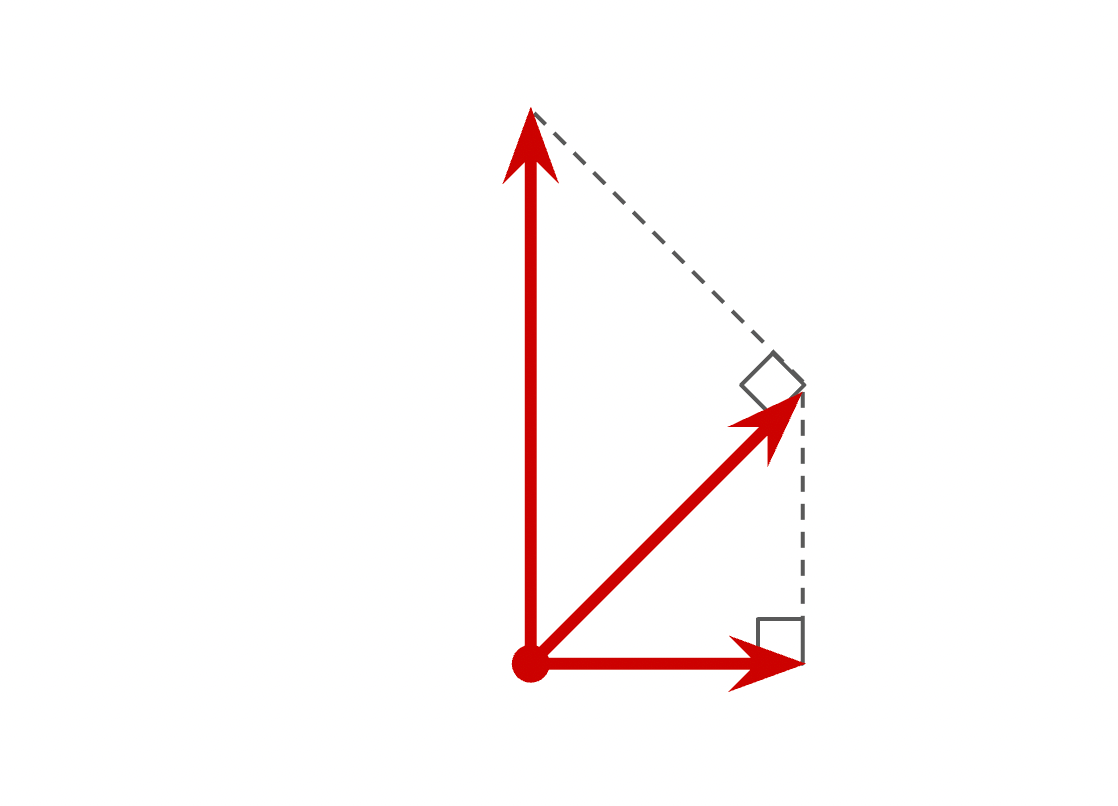
\includegraphics[width=3in]{polarization.png}
\end{center}
\vspace{0.1in}

If the first polarizer is positioned at an acute angle with respect to the light, and then the second polarizer is positioned at a complementary angle with respect to the first polarizer, some light will be horizontally polarized in the end.

Now, I have tons of polarizers, and each one also reflects 1 percent of any light that hits it---no matter its polarization or orientation---while polarizing the remaining 99 percent of the light.

I'm interested in horizontally polarizing as much of the incoming light as possible. How many polarizers should I use?


\section*{Solution:}

When polarized light passes through a polarizer, the fraction of light that is transmitted is given by the cosine of the angle between the original polarization direction and the polarizer direction.
If there are $n$ polarizers used (including the horizontal polarizer), then the maximum transmission for that particular arragement is when the polarizers are rotated equally between vertical and horizontal, and the angle between successive polarizers is $\nicefrac{\pi}{2n}$.
In this case (taking into account the 1\%\ loss at each step), the transmission is given by

\[
\left(0.99\times\cos\left(\frac{\pi}{2n}\right)\right)^n
\]

I calculated this value for $n$ between 1 and 30.
The results are in the file \texttt{Attenuated\_polarization.xlsx}.
The maximum transmission occurs for $n=11$ with a transmission of approximately 0.800.
So the solution is \fcolorbox{red}{white}{\textbf{11}}\,.


\end{document}